\documentclass[10pt,a4paper]{article}

\usepackage[margin=1in]{geometry}
\usepackage{graphicx}
\usepackage{longtable}
\usepackage[dutch]{babel}
\usepackage{url}
\usepackage{minted}
\usepackage{caption}
\usepackage{subcaption}
\usepackage{amsmath, amsthm, amssymb,amsfonts}

\usepackage[section]{placeins}

\usepackage{algorithm}
\usepackage{algpseudocode}
\newcommand*\Let[2]{\State #1 $\gets$ #2}

\usepackage{color}

\usepackage{wrapfig}

\usepackage{rotating}
\usepackage{float}

\usepackage{xypic}
\usepackage[all,color]{xy}
\xyoption{all}

\usepackage{epstopdf}
\epstopdfDeclareGraphicsRule{.tif}{png}{.png}{convert #1 \OutputFile}
\AppendGraphicsExtensions{.tif}

\usepackage{fancyhdr}
\pagestyle{fancy}
\fancyhead{}
\fancyfoot{}
\renewcommand{\headrulewidth}{0mm}
\rfoot{\thepage}    
\cfoot{}
\lfoot{CV finaal project: Snijtand Segmentatie - Christophe Van Ginneken (s0084580)}

\definecolor{bg}{rgb}{0.95,0.95,0.95}

\geometry{a4paper}

\author{Christophe Van Ginneken (s0084580) \\
	\url{Christophe.VanGinneken@student.kuleuven.be} }
\title{CV finaal project: Snijtand Segmentatie}

\begin{document}

\maketitle

\vspace{-1cm}
\section{Introductie}

In dit project bestuderen we het segmenteren van snijtanden op basis van radiografie\"en. We vertrekken hierbij van bestaande literatuur, uit de welke een strategie gekozen en ge\"implementeerd wordt. De resultaten van deze implementatie worden besproken in het kader van de cursus.

Dit rapport volgt dezelfde structuur: eerst worden enkele van de geconsulteerde rapporten kort toegelicht. Vervolgens wordt de geselecteerde strategie beschreven. De implementatie wordt tevens kort toegelicht en de uitdagingen die er in vervat zaten geanalyseerd. Tot slot worden de resultaten besproken en worden conclusies getrokken.

De belangrijkste resultaten en code voorbeelden zijn opgenomen in dit rapport, het zij in de tekst, het zij in appendices. Alle broncode die gebruikt werd in de realisatie van de gekozen strategie, is ook online beschikbaar via \url{http://github.com/MyKULCourses/cv} in de folder {\tt final}.

\section{Literatuur studie}

Enkele van de aangeboden, alsook andere, zelf gezochte artikels werden verwerkt. In deze sectie vatten we de voorgestelde strategie\"en kort samen.

\subsection{Challenges of Developing an Automated Detail Identification System}

In \cite{abdel2003challenges} wordt een strategie voorgesteld die uit twee stappen bestaat: eerst wordt een 2-ledige \emph{thresholding} methode toegepast waarna door middel van integrale projectie de individuele tanden gesegmenteerd worden. Het bepalen van de effectieve contour wordt nauwelijks beschreven en wordt opgenomen in het gedeelte over het vergelijken van de ante- en post-mortem informatie.

De 2-ledige \emph{thresholding} methode bestaat uit de toepassing van een iteratieve en een adaptieve drempelwaarde. De iteratieve drempelwaarde wordt ge\"implementeerd aan de hand van een \emph{Canny} rand detectie. De adaptieve drempelwaarde wordt gerealiseerd door middel van morfologische dilatie, toegepast op het binaire randen beeld. Op deze manier worden de pixels rond de randen gevonden. Van de overeenkomstige pixels wordt een gemiddelde grijs-waarde bepaald, die als initi\"ele drempelwaarde gebruikt wordt. Deze waarde zorgt voor een opdeling in tand- en achtergrondgebieden. Via een iteratief proces wordt deze waarde bijgesteld tot ze convergeert.

Door het toepassen van een adaptieve drempelwaarde, wordt vervolgens een binaire opdeling gemaakt tussen tanden en achtergrond. Deze drempelwaarde wordt toegepast op het originele beeld dat eerst gemaskeerd wordt met het iteratief bekomen masker.

Dit binaire beeld vorm vervolgens de basis voor het segmenteren van de individuele tanden. Hier wordt eerst gezocht naar een horizontale splitsing tussen onder- en bovenkaak. Hierbij wordt een minimale som van horizontale intensiteiten gezocht. Aangezien achtergrondgebieden zwart zijn, zal een overwegend zwarte scheidingslijn een zeer lage gesommeerde intensiteit kennen en duiden op een splitsing. Omdat deze horizontale lijn niet altijd mooi horizontaal zal zijn, wordt een rotatie van deze lijn tussen -20 en +20 graden in rekening genomen. Aangezien dit niet altijd mogelijk is, wordt voorgesteld om dit te doen voor verticale deelgebieden.

Vertrekkende van deze horizontale splitsing worden de tanden ge\"isoleerd. Hierbij wordt een gelijkaardige methode toegepast en wordt vanaf de horizontale splitsing gezocht naar rechten die loodrecht staan op de splitsing, met opnieuw in acht name van een hook tussen -20 en +20 graden, waarbij de som van de intensiteiten opnieuw minimaal is.

Het vervolg van dit artikel focust hoofdzakelijk nog op het opslaan en het terugvinden door vergelijken van de informatie over de individuele tanden.

\subsection{Active Contour Based Segmentation of Low-Contrast Medical Images}

In \cite{abdel2003challenges} wordt verwezen naar \cite{piotrowski2000active}, een artikel dat in het algemeen het probleem van contour detectie in laag-contrast medische beeldvorming aanpakt. Het artikel beschrijft enkele aspecten: eerst wordt de normalisatie van de originele beelden voorgesteld op basis van het zgn. \emph{contrast stretching}. Vervolgens wordt een initi\"le contour detectie gedaan door middel van Hough transformaties. Aan de hand van een energie functie wordt deze initi\"ele vorm vervolgens verbeterd tot het finale resultaat.

Het moet opgemerkt worden dat de segmentatie door toepassing van achtereenvolgens een Sobel filter, een drempelwaarde en Hough transformaties wel een beperking oplegt dat er bv. slechts \'e\'en tand in het beeld aanwezig mag zijn.

Het minimaliseren van de contour energie wordt gedaan door middel van \emph{simulated annealing} en kent vier fasen:

\begin{enumerate}
\item In de \emph{browsing} fase kan de vorm zeer vrij bewegen, met zeer weinig beperkingen.
\item Tijdens \emph{setting the macro-state} fase blijven contouren meer gelokaliseerd.
\item Daarna zal de contour beginnen oscilleren rond de rand van het object.
\item In de laatste fase, \emph{freezing in de local minimum} wordt door de lage \emph{temperatuur} het simulated annealing proces beperkte tot een \emph{downhill search}.
\end{enumerate}

\subsection{Tooth Contour Extraction for Matching Dental Radiographs}

De verwijzing naar actieve contouren in algemeen, laag-contrast medische beelden leidde naar \cite{chen2004tooth}, een zeer beknopt artikel waarin een strategie wordt voorgesteld op basis van actieve contour modellen of zgn. \emph{snakes} om specifiek contouren van tanden te bekomen. Omdat hierbij het probleem kan rijzen van interferentie van naburige tanden, stellen ze tevens een nieuwe dynamische energie term voor. Hierbij wordt gebruik gemaakt van gradi�nt richtingen. In het geval van tanden is dit mogelijk omdat bij een gerichte \emph{snake} de tand steeds aan de linkerkant zal liggen.

Dit artikel verwijst naar \cite{jain2004matching}, een artikel van dezelfde auteurs, en vermeldt dat de daarin voorgestelde strategie op basis van een intensiteiten distributie model, snel zal falen indien de contouren wazig zijn of er zich overlappingen voordoen. Anderzijds wordt de structurele aanpak voor de segmentatie van tanden tevens weerhouden bij de initialisatie fase.

Voor de detectie van de contouren wordt eerst gezocht naar de scheidingslijn tussen tandvlees en achtergrond. Hierdoor worden de kroon en de wortel gescheiden. Vervolgens wordt de methode van \cite{jain2004matching} toegepast om een initi\"ele \emph{snake} te bekomen. Door een convergentie naar de gradi\"ent  wordt dit initi\"ele resultaat verbeterd tot het finale resultaat.

\subsection{Dental X-ray Image Segmentation}

\cite{said2004dental} is een artikel dat duidelijk volgt op \cite{abdel2003challenges} en uitgebreider ingaat op het concept \emph{contrast stretching}, zoals ook beschreven in \cite{piotrowski2000active}.

Initieel kent het artikel een zeer lange beschrijvende inleiding, waarin de context van het segmenteren van tanden uiteen gezet wordt. Vervolgens wordt een methodologie voorgesteld. Een eerste stap bestaat uit het verbeteren van de beelden door middel van \emph{contrast stretching}. Naast de theoretische onderbouw voor \emph{contrast stretching} wordt niet verder ingegaan op de implementatie ervan. Wel wordt aangegeven dat tijdens de voorbereiding van de beelden een \emph{Top-Hat} filter nodig is om het onderscheid tussen tanden en botten mogelijk te maken.

Vervolgens wordt opgemerkt dat voor segmentatie twee strategie\"en kunnen gevolgd worden: enerzijds de extractie op basis van regionale kenmerken en anderzijds op basis van modellen. Deze laatste strategie is complexer, maar dikwijls meer succesvol.

De methodologie gaat tot slot verder met een uitermate sumiere beschrijving van de segmentatie door middel van 2D wavelets en concludeert dat deze aanpak veruit de beste is, in vergelijking met andere aanpakken.

\subsection{Matching of dental X-ray images for human identification}

In \cite{jain2004matching} wordt ook een twee-fasen methodologie voorgesteld: eerst een segmentatie van de individuele tanden en vervolgens een extractie van de effectieve contouren. De auteurs van het artikel geven zelf aan dat hun aanpak waarschijnlijk niet geschikt is voor een volledig automatische verwerking van grote sets en dat fouten in problematische situaties manueel dienen gecorrigeerd te worden. Ook adviseren ze om waar mogelijk manueel een initi\"ele aanduiding te geven van verwachte locaties, zoals voor de splitsing tussen de onder- en bovenkaak. Desalniettemin beschrijven ze een strategie die volledig geautomatiseerd kan worden.

De scheiding van onder- en bovenkaak volgt het principe dat voorgesteld werd in \cite{abdel2003challenges}, en zoekt splitsingen aan de hand van histogrammen van de horizontale en verticale intensiteiten, echter zonder de bijkomende variatie van de hellingsgraad van -20 tot +20 graden. Wel wordt het principe van de verticale banden gehanteerd. De resulterende hoogtes van de splitsingen worden vervolgens als basis genomen om een interpolerende \emph{spline} te bepalen.  Het zoeken van splitsingen tussen individuele tanden wordt vervolgens gedaan volgens rechten die loodrecht staan op deze \emph{spline}. Op basis van deze splitsingen kunnen ROI's bepaald worden die telkens (hoofdzakelijk) \'e\'en tand bedekken. 

Een ROI wordt vervolgens opgedeeld in een kroon en een wortel door middel van het identificeren van een kroon centrum halverwege de breedte en op $\frac{1}{3}$ van de top van de ROI. Via een distributiemodel van intensiteiten wordt vervolgens via een tracering van een halve cirkel de contour van de kroon bepaald. In een volgende fase wordt de wortel verder getraceerd. Hierbij wordt gewerkt met een contrast verschil omdat deze regio veel waziger is wegens de combinatie van tand en kaakbeen dat gelijkaardige intensiteiten oplevert.

De overige helft van het artikel gaat dieper in op het opslaan en vergelijken van ge\"iadentificeerde tanden.

\section{Implementatie strategie}

Voor de implementatie van dit project werd uitgegaan van \cite{jain2004matching} als basis algoritme met toepassing van  \emph{contrast stretching} zoals aangegeven in \cite{piotrowski2000active} en verder gedetailleerd in \cite{said2004dental}.

Omdat dit artikel veel geciteerd werd in de andere geconsulteerde werken en omdat het in grote lijnen een andere aanpak beschrijft dan deze die tijdens de lessen van de cursus voorgesteld werd, leek het een interessante opportuniteit om na te gaan hoe deze methodologie effectief kan presteren op basis van een implementatie binnen een kort tijdsbestek.

Vooral de aanpak om een volledige radiografie van een gebit te segmenteren in individuele ROI's wordt meermaals geciteerd. Ook worden enkele complexiteiten uit andere artikels anders opgelost. Zo wordt bv. gebruik gemaakt van een \emph{spline} functie om de splitsing tussen onder- en bovenkaak te beschrijven. Dit in tegenstelling tot de variabele hoek in \cite{abdel2003challenges}.

Zoals aangegeven in \cite{chen2004tooth} verwachten we inderdaad dat er mogelijke problemen zullen optreden bij beelden waarbij de contouren wazig zijn of waar er zich overlappingen voordoen. Dit laatste is niet ongewoon bij vervormingen en komt in een radiografie tot uiting door overlappingen van de beelden van de individuele tanden.

\section{Implementatie}

In dit deel bespreken we de implementatie van de gekozen strategie. Hierbij bekijken we eerst de setup van het project met de verdeling van verantwoordelijkheden over gekozen technologie\"en en de structurele opdeling in scripts.

Vervolgens doorlopen we de implementatie chronologisch. Hierbij bespreken we de aanpak zoals deze voorgesteld werd in de literatuur en geven we aan bepaalde aannames werden gedaan of waar aanpassingen werden doorgevoerd om bepaalde problemen te verhelpen.

\subsection{Setup}

De resulterende code is hoofdzakelijk geschreven in Python, maakt gebruik van de OpenCV, NumPy en SciPy bibliotheken. Daarnaast werd geopteerd om de co\"ordinatie en aansturing van deze code te doen vanuit een doel-geori\"enteerde {\tt Makefile}. Hierdoor is er een sterke scheiding tussen configuratie en aansturing enerzijds en algoritme en uitvoering anderzijds. Zaken als bepalen welke bestanden geladen moeten worden of welke logica dient uitgevoerd te worden is op deze manier gecentraliseerd en niet verspreid over de verschillende Python bestanden.

Voor elke fase of handeling die uitgevoerd wordt, is een apart Python script voorzien. Deze zijn opgezet als modules, maar kunnen ook op zich uitgevoerd worden. In dit laatste geval zal het script zijn functionaliteit uitvoeren en het resultaat interactief laten zien op het scherm. Deze werking wordt geactiveerd indien er geen uitvoerbestand wordt meegegeven aan de oproep.

Indien dit laatste wel wordt gedaan, is dit de naam van een {\tt Matlab} bestand met extensie {\tt .mat}. In plaats van de resultaten te visualiseren, worden deze nu opgeslagen in dit bestand. Deze bestanden worden tevens doorgegeven aan de volgende fase, waardoor er voor elke fase een onafhankelijke set van data- en uitvoer bestanden ontstaan. Het {\tt Matlab} formaat werd gekozen om wille van interoperabiliteit. Zo zijn de scripts om grafieken, zoals histogrammen, te visualiseren gerealiseerd als {\tt Matlab} scripts. Hierdoor zijn deze grafieken in dit verslag visueel conform aan geldende standaarden en kon ervaring op dit vlak hergebruikt worden.

Tot slot zijn er naast de interactieve manier om de resultaten te bekijken, ook overeenkomstige Python scripts gemaakt die de visualisatie realiseren naar een bestand.

De hele setup is visueel weergegeven in figuur \ref{fig:setup}: van boven naar onder is de implementatie strategie stap voor stap weergegeven in de vorm van rechthoeken met de naam van het overeenkomstige Python of Octave script. Verticale pijlen duiden de logische opeenvolging aan en geven tevens aan welke bestanden uit een vorige fase gebruikt worden om verder te gaan. Horizontale pijlen geven de mogelijkheden tot visualisatie.

\begin{figure}
\centering
\[ \entrymodifiers={+++[F-]}
\SelectTips{cm}{}
\xymatrix {
	*{origineel} 										\ar[d]_{\tt 01.tif} \\
	\parbox{3.75cm}{\centering crop\_image.py} 					\ar[d]_{\tt 01\_crp.tif} \\
	\parbox{3.75cm}{\centering create\_histogram.py} 			\ar[d]_{\tt 01\_crp.tif}^{\tt 01\_crp\_histogram.mat}
		\ar[rr]^{\tt 01\_crp\_histogram.mat} &*{\hspace{2cm}} & \parbox{3.75cm}{\centering plot\_histogram.m} \\
	\parbox{3.75cm}{\centering create\_enhanced\_image.py} 		\ar[d]	_{\tt 01\_crp\_enh.tif}	
	&*{\hspace{2cm}} & \parbox{3.75cm}{\centering plot\_jaw\_histograms.m} \\
	*+++[F=]{\parbox{3.75cm}{\centering jaw\_split.py}} 					\ar[d]_{\tt 01\_crp\_enh.tif}^{\tt 01\_crp\_enh\_jaw\_split.mat}
		\ar[rru]^{\tt 01\_crp\_enh\_jaw\_split.mat}  \ar[rr]^{\tt 01\_crp\_enh\_jaw\_split.mat}_{\tt 01\_crp\_enh.tif}
		&*{\hspace{2cm}} & \parbox{3.75cm}{\centering visualize\_jaw\_split.m} \\
	*+++[F=]{\parbox{3.75cm}{\centering teeth\_isolation.py}} 				\ar[d]	^{\tt 01\_crp\_enh\_teeth\_iso.mat}
		\ar[rr]^{\tt 01\_crp\_enh\_teeth\_iso.mat}_{\tt 01\_crp\_enh\_jaw\_split.mat} &*{\hspace{2cm}} & \parbox{3.75cm}{\centering visualize\_teeth\_isolation.py} \\
	*+++[F=]{\parbox{3.75cm}{\centering roi.py}}							\ar[d]	_{\tt 01\_crp\_enh.tif}^{\tt 01\_crp\_enh\_roi.mat}
		\ar[rr]^{\tt 01\_crp\_enh\_roi.mat}_{\tt 01\_crp\_enh\_teeth\_iso.mat} &*{\hspace{2cm}} & \parbox{3.75cm}{\centering visualize\_roi.py} \\
	*+++[F=]{\parbox{3.75cm}{\centering contours.py}}
		\ar[rr]^{\tt 01\_crp\_enh\_contours.mat}_{\tt 01\_crp\_enh\_roi.mat}
		\ar[d]^{\tt 01\_crp\_enh\_contours.mat}_{\tt 01\_crp\_enh\_roi.mat} &*{\hspace{2cm}} &  \parbox{3.75cm}{\centering visualize\_contours.py} \\
	\parbox{3.75cm}{\centering create\_masks.py}
		\ar[rr]^{\tt 01\_crp\_enh\_masks.mat} &*{\hspace{2cm}} &  \parbox{3.75cm}{\centering visualize\_masks.py} \\
}
\]
\caption{Overzicht setup en werking}
\label{fig:setup}
\end{figure}

Het originele beeld wordt eerst voorbereid. Hierbij wordt het algemeen bijgesneden ({\tt crop\_image.py}) tot een beeld dat hoofdzakelijk de tanden bevat. Vervolgens wordt van dit beeld een histogram van de intensiteiten gemaakt ({\tt create\_histogram.py}). Aan de hand van dit histogram wordt het beeld vervolgens verbeterd ({\tt create\_enhanced\_image.py}). Dit zijn algemene acties die het beeld voorbereiden voor het effectieve algoritme.

Dit algoritme bestaat uit 4 fasen. Deze zijn in figuur \ref{fig:setup} weergegeven met dubbele omkaderende lijnen. Eerst wordt een splitsing gemaakt tussen de boven- en onderkaak ({\tt jaw\_split.py}). Dan worden voor elk van deze kaken, splitsingen gezicht tussen de vier middelste tanden, waardoor deze ge\"isoleerd worden ({\tt teeth\_isolation}). Op basis van deze splitsingen worden dan rechthoekige afbakeningen van de interessante regio gemaakt, de zgn. \emph{Region Of Interest of ROI} ({\tt roi.py}). Tot slot wordt binnen deze ROI's gezocht naar de contour van de tand ({\tt contours.py}).

De opdracht voorziet dat binaire maskeringen aangemaakt worden. Een laatste stap in het proces voorziet de generatie van zulke maskeringen ({\tt create\_masks.py}).

\subsection{Voorbereiding}

Vooralleer de segmentatie en contour afbakening kan gebeuren, is het aangewezen om het originele beeld voor te bereiden. De originele beelden zijn zeer ruim in functie van de scope van de opdracht. De opdracht focust op de acht snijtanden, daar waar de originele beelden de volledige kaken beslaan. Daarom werd besloten om als eerste stap een zeer ruwe ROI te bepalen, een zgn. macro-ROI.

Vervolgens dient ook het contrast verbeterd te worden. Hiervoor werd de techniek \emph{contrast stretching} uit  \cite{piotrowski2000active} en \cite{said2004dental} gehanteerd.

\subsubsection{Bepalen macro-ROI}

De originele beelden laten toe om de sterke structurele gelijkenissen uit te buiten en het volledige beeld te herleiden tot een kleiner beeld waar zich alleen de zone op bevindt die belangrijk is in dit project. Zonder te zoeken naar optimale maten, werd een ruwe bijsnijding ge\"implementeerd die het beeld herleidde tot een centrale regio van 700 pixels breed en 1100 pixels hoog\footnote{De originele beelden zijn 3023 breed en 1597 hoog.}.

Zoals blijkt uit het overzicht van de voorbereide originele beelden in appendix \ref{appendix:prepared-originals}, kan deze bijsnijding eigenlijk nog verbeterd worden en kan vooral aan de bovenkant nog meer onnuttig beeldmateriaal verwijderd worden. Er is geopteerd om deze geleide operaties zo algemeen mogelijk uit te voeren om zo min mogelijke manuele interferentie te noodzaken. Hierdoor zijn de voorbereidingen redelijk ruw, maar zo weerspiegelen hopelijk de resultaten de kwaliteiten van de strategie in een geautomatiseerde omgeving waar zo min mogelijk interventie nodig is.

We merken op dat een aantal van de originele beelden problematische eigenschappen vertonen zoals schaduwen, corrigerende beugels en blokjes. Daarnaast zijn er ook een aantal beelden met sterk vervormde structuren.

\subsubsection{Verbeteren van het contrast}

Radiografie-beelden zijn gekenmerkt door een veelheid aan grijstinten en wazige overgangen. Omdat we op basis van histogrammen van intensiteiten splitsingen willen gaan bepalen, is het belangrijk dat er een duidelijk onderscheid is tussen donkere en lichte zones. Om deze reden is het belangrijk om te zorgen voor een accentuering van het contrast, waarbij donkere zones expliciet donkerder gemaakt worden lichtere zones lichter. Een techniek die dit doet is het zogenaamde \emph{contrast stretching}.

Zoals de naam doet vermoeden trachten we bij \emph{contrast stretching} het contrast dat er is zo uit te rekken, dat het nadrukkelijker aanwezig is. Om dit te doen, werken we met een histogram van de intensiteiten van de grijs-waarden en defini�ren we een transformatie van deze intensiteiten. Figuur \ref{fig:contrast-stretching-histograms} toont het histogram voor en na \emph{contrast stretching}. Het is duidelijk dat de intensiteiten nu als het ware uitgerokken zijn over het volledige spectrum en dat de stretching vooral in de middelste zone gebeurd is. Merk op dat door het uitrekken er ook gaten ontstaan.

\begin{figure}
\centering
\begin{subfigure}{.49\textwidth}
  \centering
  \includegraphics[width=.9\linewidth]{../01_crp_histogram.eps}
  \caption{Origineel}
  \label{fig:original-histogram}
\end{subfigure}
\begin{subfigure}{.49\textwidth}
  \centering
  \includegraphics[width=.9\linewidth]{../01_crp_enh_histogram.eps}
  \caption{Na verbetering}
  \label{fig:enhanced-histogram}
\end{subfigure}
\label{fig:contrast-stretching-histograms}
% \caption{Histogrammen voor en na contrast stretching van {\tt 01_crp.tif}}
\end{figure}

Als transformatiefunctie werd een \emph{sigmoid} functie gebruikt weergegeven door vergelijking \ref{eq:sigmoid}.

\begin{equation} \label{eq:sigmoid}
\frac{255}{1+e^{-\frac{I - \beta}{\alpha}}}
\end{equation}

Figuur \ref{fig:sigmoid} toont het verloop van deze transformatie.

\begin{figure}
%  \includegraphics[width=.5\linewidth]{../01_crp_sigmoid.eps}
%  \caption{Sigmoid-gebaseerde normalisatie transformatie voor {\tt 01_crp.tif}}
  \label{fig:original-histogram}
\end{figure}



Figuur \ref{fig:preparation} geeft een visueel overzicht van de evolutie van origineel beeld tot bijgesneden beeld met verbeterd contrast.

\begin{figure}
\centering
\begin{subfigure}{.32\textwidth}
  \centering
  \includegraphics[width=.9\linewidth]{../images/01.tif}
  \caption{Origineel beeld}
  \label{fig:original}
\end{subfigure}
\begin{subfigure}{.32\textwidth}
  \centering
  \includegraphics[width=.9\linewidth]{../01_crp.tif}
  \caption{Bijgesneden beeld}
  \label{fig:cropped}
\end{subfigure}
\begin{subfigure}{.32\textwidth}
  \centering
  \includegraphics[width=.9\linewidth]{../01_crp_enh.tif}
  \caption{Verbeterd contrast}
  \label{fig:cropped}
\end{subfigure}
\caption{Evolutie tijdens de voorbereiding van {\tt 01.tif}.}
\label{fig:preparation}
\end{figure}


\subsection{Segmentatie}

TODO

\subsection{Contour bepaling}

TODO

\section{Resultaten}

TODO

\section{Conclusies}

TODO

\bibliographystyle{alpha}
\bibliography{references}

\newpage

\appendix

\section{Voorbereide originele beelden}
\label{appendix:prepared-originals}

\begin{figure}[H]
\includegraphics[width=\linewidth]{../prepared.png}
\caption{Voorbereide originele beelden.}
\label{fig:prepared-originals}
\end{figure}

\section{Boven- en onder kaak-splitsing}
\label{appendix:jaw-split}

\begin{figure}[H]
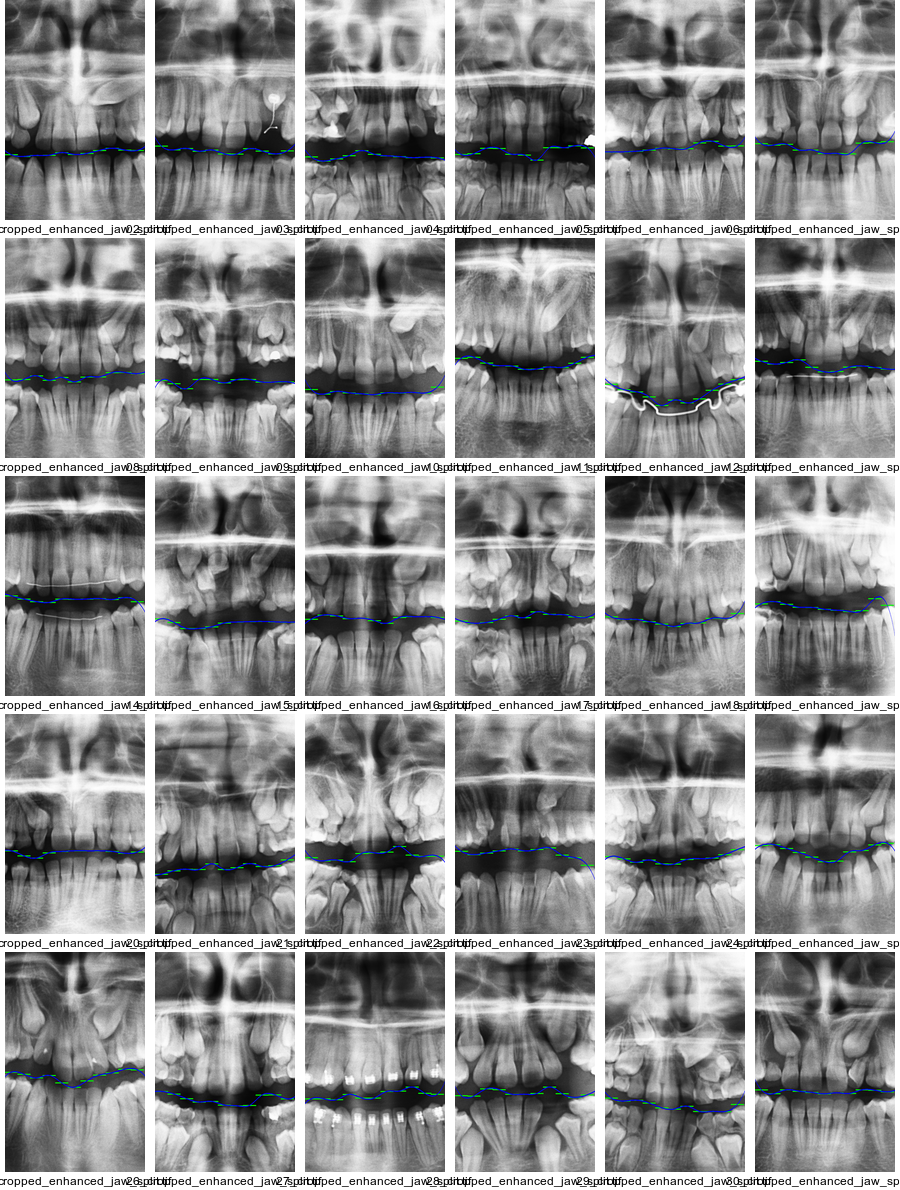
\includegraphics[width=\linewidth]{../jaw_splits.png}
\caption{Splitsing van onder- en bovenkaak.}
\label{fig:jaw-splits}
\end{figure}

\section{Individuele snijtand segmentatie}
\label{appendix:teeth-segmentation}

\begin{figure}[H]
\includegraphics[width=\linewidth]{../teeth_iso.png}
\caption{Splitsing van individuele snijtanden.}
\label{fig:teeth-isolation}
\end{figure}

\section{ROI's}
\label{appendix:rois}

\begin{figure}[H]
\includegraphics[width=\linewidth]{../roi.png}
\caption{ROI's}
\label{fig:rois}
\end{figure}

\section{Resulterende contouren}
\label{appendix:contours}

\begin{figure}[H]
\includegraphics[width=\linewidth]{../contours.png}
\caption{Contourss}
\label{fig:contours}
\end{figure}

\end{document}
